\chapter{Background or Project Scope}

\section{Introduction} % Section 2.1
The healing process does not end after surgery is complete, but instead it is often a long effort for weeks or months post-operation. Furthermore, it is not just the physical health of the patient which must be considered, but also and perhaps equally important their mental health and quality of life moving forward. In recent decades it has become clearer to medical professionals that extended monitoring following operations greatly impacts the results of surgeries in a positive manner, as stated in \cite{d2014defining}. Of course, there are multiple factors affecting the extent to which complications will arise in a patient after receiving surgery, such as their age, previous health issues, or conditions which may develop in parallel to the primary diagnosis even if they are in fact unrelated. In particular, the elderly are quite vulnerable to more complications, as stated by \cite{kare2024post}, specifically referring to elderly patients who underwent hip fracture surgery. Such complications affect quality of life longterm as well as general ability to function normally, not just physical health, degree of recovery, and survivability \cite{kare2024post}.

The role of the surgeon in the postoperative context is to firstly make sure the patient is receiving the necessary support to sustain a healthy balance in their body, and do whatever they can to avoid the development of and complications that may appear as a result of the procedure. Should any complications arise despite the medical staff's best efforts, it is then the surgeon's responsibility to recognise the signs pointing to the development of said complications and take appropriate actions to quickly and effectively manage them, allowing the patient to recover to their preoperative state eventually \cite{Surwit_Tam_2008}

\section{Clinical significance of monitoring each vital sign post-surgery} % Section 2.2
Vital signs give a rich picture of patient condition post surgery, providing medical staff with the information required to adequately care for the patient. Different measurements have varying significance depending on the stage of recovery the patient finds themselves in, however they should be continuously measured to provide history and an indication of trends to clearly show the progress of the patient's condition. Immediately after surgery measurements must be taken often as that is the most critical stage of the recovery process. In the beginning, vitals such as respiratory rate and blood pressure are vastly more important due to their indication of how the patient is recovering from anesthesia, but once they sufficiently recover from it pulse rate is a better indicator of the volume of blood in the circulatory system of a patient \cite{Surwit_Tam_2008}


\section{Role of IoT in vital sign monitoring} % Section 2.3
\section{Communication protocols in IoT-based monitoring} % Section 2.4
This section explores the communication protocols relevant to IoT-based monitoring of post-operative patients, focusing on Bluetooth and LoRaWAN. Reliable and efficient data transmission is crucial in this context, where vital signs such as heart rate, temperature, and blood pressure need to be collected with minimal power consumption and transmitted securely over short or long distances.

LoRa is a wireless modulation technique derived from chirp spread spectrum technology. It enables long-distance, low-power communication by encoding information on radio waves using chirp pulses. This makes it robust against interference and highly suitable for IoT applications that transmit small data packets at low bit rates \cite{what_are_lora_lorawan}. Compared to technologies like WiFi, Bluetooth, or ZigBee, LoRa supports data transmission over significantly longer distances, particularly in sub-gigahertz bands, making it well suited for both indoor hospital and outdoor monitoring environments \cite{lora_documentation}.
\begin{figure}[H]
\centering
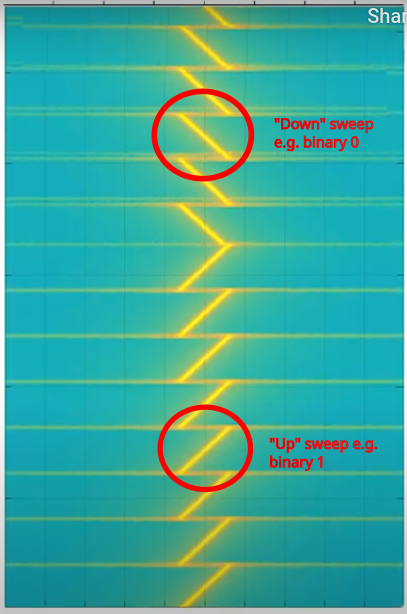
\includegraphics[width=0.5\textwidth]{images/chirp_spread_spectrum_labeled.png}
\caption{Example of a chirp spread spectrum transmission, highlighting the up and down sweeps which represent binary 1 and 0. \cite{Wenner2017-hd}}
\label{fig:chirp_spread_spectrum_labeled}
\end{figure}

LoRaWAN builds upon the LoRa physical layer by adding a media access control (MAC) protocol. It defines how devices connect, how data is encrypted, and how the network is managed. LoRaWAN is designed for ultra-low-power operations, allowing devices to last several years on small batteries, and offers deep indoor penetration, which is particularly valuable in hospital settings where walls and medical equipment can attenuate signals \cite{lora_documentation}.

To assess the suitability of LoRaWAN, it is important to compare it to other LPWAN technologies, including SigFox, NB-IoT, and LTE-M. Below is a table summarising their main advantages and disadvantages.
\begin{table}[H]
\centering
\caption{LPWAN technologies - Advantages \& Disadvantages \cite{sigfox_advantages_disadvantages, nbiot_advantages_disadvantages, ltem_advantages_disadvantages, lorawan_advantages_disadvantages}}
\begin{tabularx}{\textwidth}{l X X}
\toprule
\textbf{Technology} & \textbf{Advantages} & \textbf{Disadvantages} \\
\midrule
LoRaWAN &
\begin{itemize}
	\item Long range
	\item Low power consumption
	\item Adaptive data rates
	\item Deep indoor penetration
	\item Low cost
\end{itemize}
&
\begin{itemize}
	\item Limited by duty cycle
	\item Unsuitable for real-time or low latency applications
\end{itemize}
\\
SigFox &
\begin{itemize}
	\item Lightweight protocol
	\item Minimal overhead
	\item Long battery life
	\item Wide coverage
	\item Underground support
\end{itemize}
&
\begin{itemize}
	\item One-way communication
	\item Limited data rates
	\item One operator per country
\end{itemize}
\\
NB-IoT &
\begin{itemize}
	\item High scalability
	\item Robust QoS
	\item Extended range
	\item Structure penetration
	\item Backed by operators
\end{itemize}
&
\begin{itemize}
	\item Licensed spectrum costs
	\item Lower data rates than LTE-M
	\item No roaming support
\end{itemize}
\\
LTE-M &
\begin{itemize}
	\item High data rates
	\item Excellent coverage
	\item LTE network integration
	\item Efficient power use
\end{itemize}
&
\begin{itemize}
	\item Higher costs
	\item Firmware updates consume power
	\item Not for high-volume data
\end{itemize}
\\
\bottomrule
\end{tabularx}
\label{tab:lpwan_adv_disadv}
\end{table}



Bluetooth is also widely used in medical IoT devices. While it offers short-range connectivity and is well-suited for personal health devices like heart rate monitors and themometers, its power consumption and range limit its usefulness for hospital-wide or remote patient monitoring. Bluetooth Low Energy (BLE) improves power efficiency and is increasingly integrated into wearable medical devices.

section{Commercially available medical devices} % Section 2.5

\subsubsection{Testing}
While the focus of this project was not to benchmark the LoRaWAN protocol itself, preliminary simulations were conducted to validate its suitability for post-operative monitoring applications. A single base station scenario was simulatedusing open-source software provided by Lancaster University \cite{lancaster_uk_simulation_software}. The simulation was adapted to run on Python 3, and tests were conducted with 100 and 200 node configurations.

The key objective was to confirm that LoRaWAN could handle multiple nodes transmitting small amounts of data at low power over long distances. Results showed that as the number of nodes doubled, the number of collisions also increased, which is consistent with LoRaWAN's access behaviour. Despite the increase in collisions, transmission efficiency per node remained stable, and energy consumption scaled predictably with the node count. These outcomes support the choice of LoRaWAN as a communication backbone in the system, balancing scalability and energy efficiency in a medical monitoring context.

\section{Integration with custom IoT systems} % Section 2.6
\section{Summary} % Section 2.7
Summarise what was said in this chapter and link with the next chapter.
